% !TEX program = lualatex
\documentclass[lualatex,ja=standard]{bxjsarticle}

\usepackage{graphicx}   % 画像の挿入
\usepackage{subcaption} % 複数図の並列配置（subfigure）
\usepackage{tikz}       % TikZ で代替サンプル画像を生成

\title{図のサンプル}
\author{LaTeX サンプル}
\date{\today}

\begin{document}

\maketitle

% -------------------------------------------------------------------
% 外部画像ファイルの挿入
% -------------------------------------------------------------------
\section{外部画像の挿入}

\texttt{\textbackslash includegraphics} で画像ファイル（PNG / JPG / PDF）を挿入します。
同じディレクトリに \texttt{sample.png} などの画像を配置してください。

\begin{verbatim}
\begin{figure}[h]
  \centering
  
\includegraphics[width=0.5\linewidth]{sample.png}
  \caption{サンプル画像}
  \label{fig:sample}
\end{figure}
\end{verbatim}

\begin{figure}[h]
  \centering
  
\includegraphics[width=0.5\linewidth]{sample.png}
  \caption{サンプル画像}
  \label{fig:sample}
\end{figure}

% -------------------------------------------------------------------
% TikZ で生成したインライン図
% -------------------------------------------------------------------
\section{TikZ で生成した図}

外部ファイルなしでも \texttt{tikzpicture} 環境で図を描けます。

\begin{figure}[h]
  \centering
  \begin{tikzpicture}
    \draw[thick, blue, fill=blue!20] (0,0) rectangle (3,2);
    \draw[thick, red,  fill=red!20]  (1,0.5) circle (0.7);
    \node at (1.5, 2.3) {矩形と円};
  \end{tikzpicture}
  \caption{TikZ による図の例}
  \label{fig:tikz}
\end{figure}

% -------------------------------------------------------------------
% 図の配置オプション
% -------------------------------------------------------------------
\section{配置オプション}

\texttt{figure} 環境の位置指定オプション:

\begin{description}
  \item[\texttt{h}] できるだけその場所（here）に配置
  \item[\texttt{t}] ページ上部（top）に配置
  \item[\texttt{b}] ページ下部（bottom）に配置
  \item[\texttt{H}] 強制的にその場所に配置（\texttt{float} パッケージ必要）
\end{description}

% -------------------------------------------------------------------
% 図の幅・スケール指定
% -------------------------------------------------------------------
\section{サイズ指定}

\begin{itemize}
  \item \texttt{width=0.5\textbackslash linewidth} --- ページ幅の 50\%
  \item \texttt{width=8cm} --- 絶対指定
  \item \texttt{scale=0.8} --- 元のサイズに対する倍率
  \item \texttt{angle=90} --- 回転（度）
\end{itemize}

% -------------------------------------------------------------------
% 複数の図を横並び（subcaption）
% -------------------------------------------------------------------
\section{複数図の並列配置 (subfigure)}

\begin{figure}[h]
  \centering
  \begin{subfigure}[b]{0.45\linewidth}
    \centering
    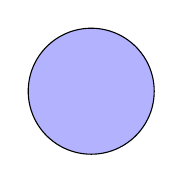
\begin{tikzpicture}
      \draw[fill=blue!30] (0,0) circle (0.8);
    \end{tikzpicture}
    \caption{図 (a): 円}
    \label{fig:circle}
  \end{subfigure}
  \hfill
  \begin{subfigure}[b]{0.45\linewidth}
    \centering
    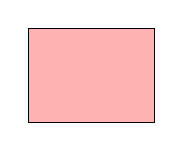
\begin{tikzpicture}
      \draw[fill=red!30] (0,0) rectangle (1.6,1.2);
    \end{tikzpicture}
    \caption{図 (b): 矩形}
    \label{fig:rect}
  \end{subfigure}
  \caption{2つの図を並列表示}
  \label{fig:two}
\end{figure}

図~\ref{fig:circle} は円、図~\ref{fig:rect} は矩形です。

\end{document}